\documentclass{article}
\usepackage{tikz}
\usetikzlibrary{calc}

\begin{document}

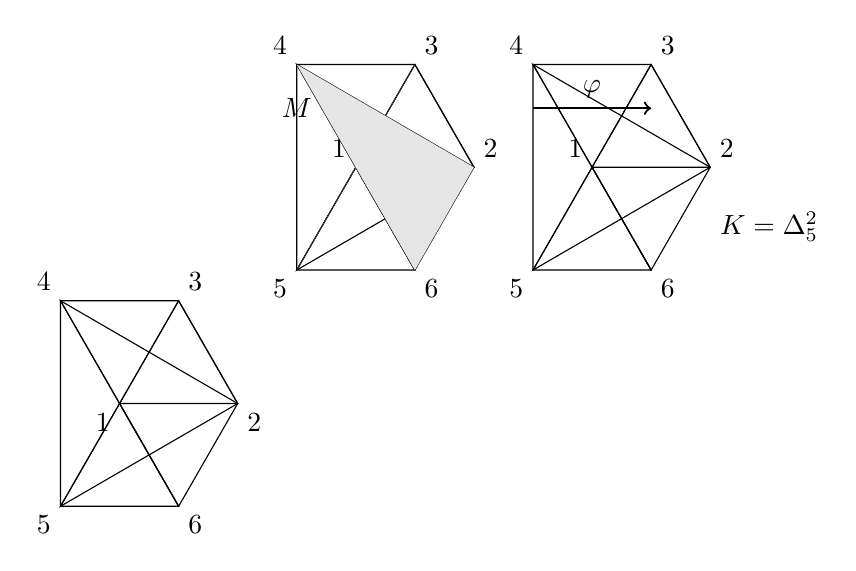
\begin{tikzpicture}[scale=1.5]
    % Define coordinates for the vertices of the 5-simplex
    \coordinate (A) at (0,0);
    \coordinate (B) at (1,0);
    \coordinate (C) at (0.5,0.87);
    \coordinate (D) at (-0.5,0.87);
    \coordinate (E) at (-0.5,-0.87);
    \coordinate (F) at (0.5,-0.87);

    % Draw the 5-simplex
    \draw (A) -- (B) -- (C) -- (D) -- (E) -- (F) -- cycle;
    \draw (A) -- (C) -- (E) -- cycle;
    \draw (B) -- (D) -- (F) -- cycle;
    \draw (A) -- (D) -- (F) -- cycle;
    \draw (B) -- (C) -- (E) -- cycle;

    % Label the vertices
    \node at (A) [below left] {$1$};
    \node at (B) [below right] {$2$};
    \node at (C) [above right] {$3$};
    \node at (D) [above left] {$4$};
    \node at (E) [below left] {$5$};
    \node at (F) [below right] {$6$};

    % Define coordinates for the vertices of the pseudomanifold M
    \coordinate (A') at (2,2);
    \coordinate (B') at (3,2);
    \coordinate (C') at (2.5,2.87);
    \coordinate (D') at (1.5,2.87);
    \coordinate (E') at (1.5,1.13);
    \coordinate (F') at (2.5,1.13);

    % Draw the pseudomanifold M
    \draw (A') -- (B') -- (C') -- (D') -- (E') -- (F') -- cycle;
    \draw (A') -- (C') -- (E') -- cycle;
    \draw (B') -- (D') -- (F') -- cycle;
    \draw (A') -- (D') -- (F') -- cycle;
    \draw (B') -- (C') -- (E') -- cycle;

    % Label the vertices of M
    \node at (A') [above left] {$1$};
    \node at (B') [above right] {$2$};
    \node at (C') [above right] {$3$};
    \node at (D') [above left] {$4$};
    \node at (E') [below left] {$5$};
    \node at (F') [below right] {$6$};

    % Define coordinates for the vertices of K = Δ^2_5
    \coordinate (A'') at (4,2);
    \coordinate (B'') at (5,2);
    \coordinate (C'') at (4.5,2.87);
    \coordinate (D'') at (3.5,2.87);
    \coordinate (E'') at (3.5,1.13);
    \coordinate (F'') at (4.5,1.13);

    % Draw the graph K = Δ^2_5
    \draw (A'') -- (B'') -- (C'') -- (D'') -- (E'') -- (F'') -- cycle;
    \draw (A'') -- (C'') -- (E'') -- cycle;
    \draw (B'') -- (D'') -- (F'') -- cycle;
    \draw (A'') -- (D'') -- (F'') -- cycle;
    \draw (B'') -- (C'') -- (E'') -- cycle;

    % Label the vertices of K
    \node at (A'') [above left] {$1$};
    \node at (B'') [above right] {$2$};
    \node at (C'') [above right] {$3$};
    \node at (D'') [above left] {$4$};
    \node at (E'') [below left] {$5$};
    \node at (F'') [below right] {$6$};

    % Draw the arrow indicating the mapping φ
    \draw[->, thick] (3.5,2.5) -- (4.5,2.5) node[midway, above] {$\varphi$};

    % Draw the label for M
    \node at (1.5,2.5) {$M$};

    % Draw the label for K
    \node at (5.5,1.5) {$K = \Delta^2_5$};

    % Shade the regions of M
    \fill[gray!20] (A') -- (C') -- (E') -- cycle;
    \fill[gray!20] (B') -- (D') -- (F') -- cycle;
    \fill[gray!20] (A') -- (D') -- (F') -- cycle;

\end{tikzpicture}

\end{document}